\section{Benutzeroberfläche}
\label{sec:Benutzeroberfläche}


Dieser Abschnitt beschäftigt sich mit der grundlegenden Gestaltung der Benutzeroberfläche für die unterschiedlichen Nutzer. Zunächst


\begin{tabular}{p{1.5cm}p{14.5cm}}
 /B10/	& Fensterlayout, Dialogstruktur und Mausbedienung entsprechen dem Windows-Gestaltungs-Regelwerk. \\[0.25cm]	 
\end{tabular}

\begin{tabular}{p{1.5cm}p{14.5cm}}
 /B11/	& Sämtliche Daten sind passwortgeschützt und dürfen nur von autorisierten Mitarbeitern des Lehrstuhls bearbeitet werden. \\[0.25cm]	 
\end{tabular}


\subsection{Bildschirmlayout}

\begin{tabular}{p{1.5cm}p{14.5cm}}
 /B20/	& Übersichtliche Gestaltung der Funktionen und intuitive Nutzung durch ein angepasstes Bildschirmlayout. \\[0.25cm]	 
\end{tabular}

\begin{tabular}{p{1.5cm}p{14.5cm}}
 /B30/	& Standardmäßig startet das Programm mit einer Suchmaske. Weitere Funktionen sind via Tabs und einer Anmeldung erreichbar. \\[0.25cm]	 
\end{tabular}

\begin{tabular}{p{1.5cm}p{14.5cm}}
 /BF40/	& Individuelle Anpassungsfähigkeit des Bildschirmlayouts an die Fenstergröße sollte möglich sein. \\[0.25cm]	 
\end{tabular}

\subsection{Drucklayout}

\begin{tabular}{p{1.5cm}p{14.5cm}}
 /B50/	& Nicht Angemeldete Nutzer können über die Auswahl verschiedener Lehrveranstaltungen einen Stundenplan im PDF-Format in Din-A4 Größe erzeugen lassen. \\[0.25cm]	 
\end{tabular}

\begin{tabular}{p{1.5cm}p{14.5cm}}
 /B60/	& Die Hausverwaltungsnutzer können folgende Raumpläne im PFD-Format und Din-A4 Größe erzeugen lassen. \\[0.25cm]	 
\end{tabular}

\begin{tabular}{p{1.5cm}p{14.5cm}}
 /B70/	& Mitarbeiter der Lehrstühle können personen- oder lehrstuhlbezogene Wochenpläne in ein PDF-Format exportieren in Din-A4 Größe. \\[0.25cm]	 
\end{tabular}

Hier einige Beispiele zur Ausgabe des Stundenplans für Studenten, Dozenten und Lehrstühle:
\begin{figure}[H]
\begin{center}
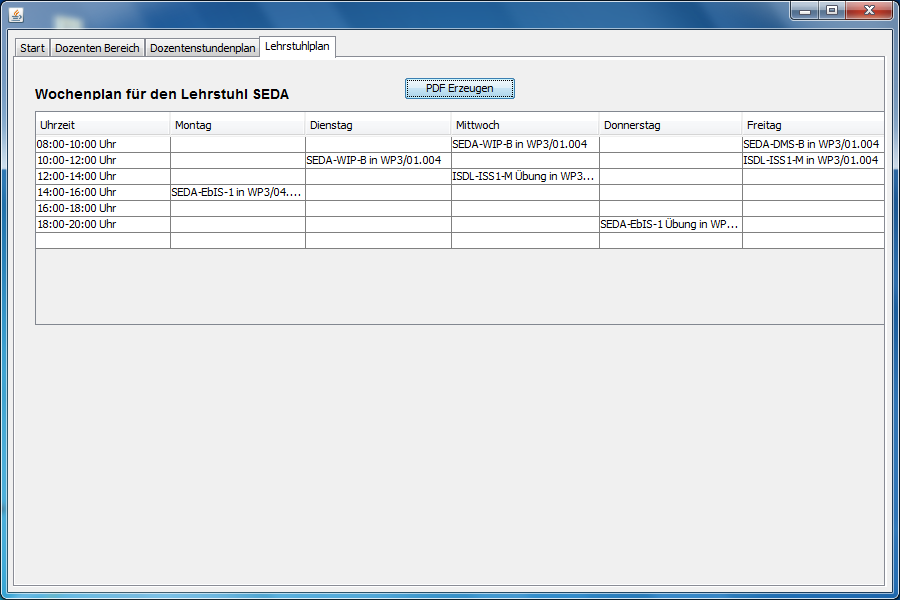
\includegraphics[width=120mm]{images/section_7/DozentenLehrstuhlplan.PNG}
\caption{Lehrstuhlplan}
\label{img:LehrstuhlplanDoz}
\end{center}
\end{figure}

\begin{figure}[H]
\begin{center}
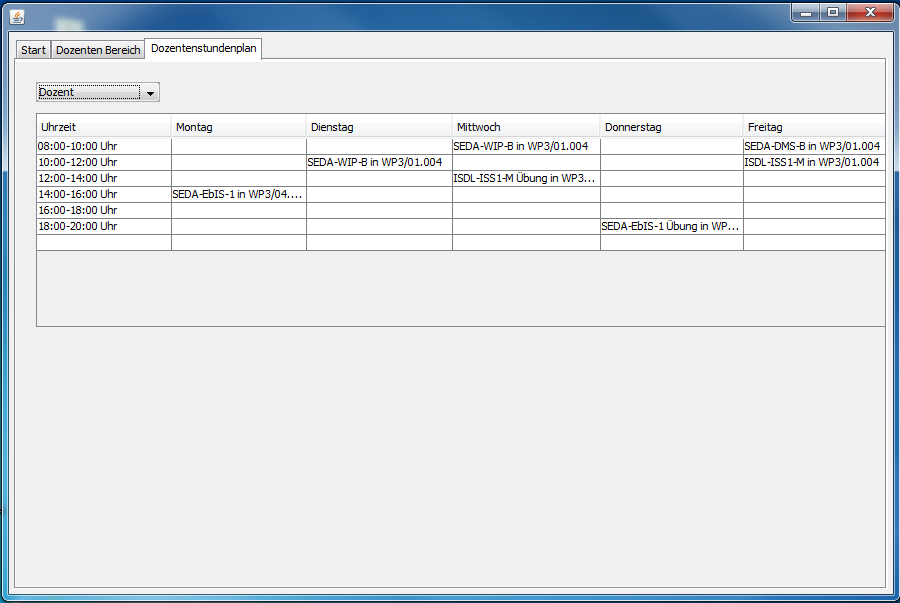
\includegraphics[width=120mm]{images/section_7/DozentenStundenplan.PNG}
\caption{Dozentenstundenplan}
\label{img:StundenplanDoz}
\end{center}
\end{figure}

\begin{figure}[H]
\begin{center}
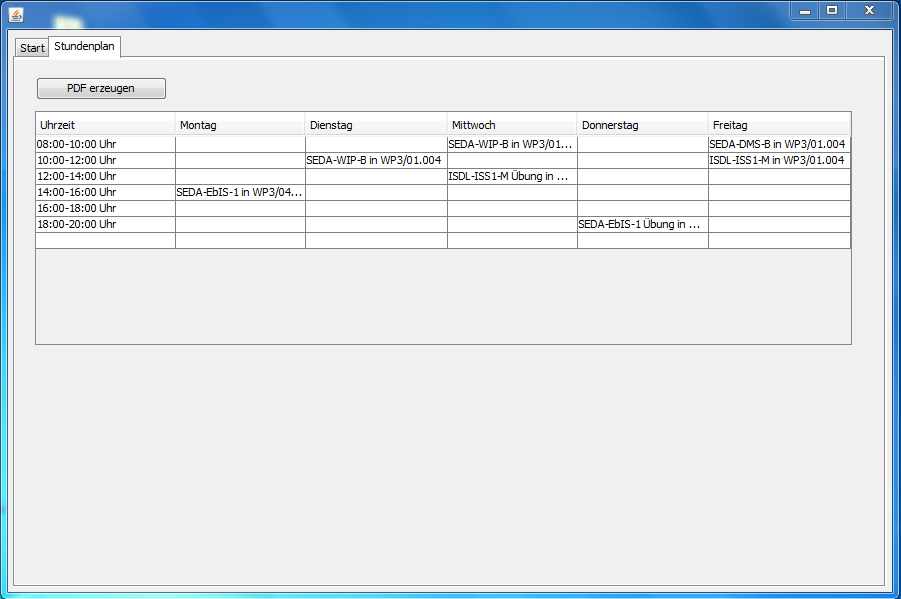
\includegraphics[width=120mm]{images/section_7/HauptseiteAlleStundenplan.PNG}
\caption{Stundenplananzeige, rollenunabhängig}
\label{img:stundenplanAlle}
\end{center}
\end{figure}
 
\subsection{Tastaturbelegung}

\begin{tabular}{p{1.5cm}p{14.5cm}}
 /B80/	& Die Bedienoberfläche ist auf eine Bedienung mittels Tastatur und Maus auszulegen. Benutzer in der Studentenrolle können keine Eingaben mittels der Tastatur vornehmen. Dozenten und die Hausverwaltung brauchen die Tastatur um verschiedene Funktionen auszuführen. \\[0.25cm]	 
\end{tabular}

\begin{tabular}{p{1.5cm}p{14.5cm}}
 /BF81/	& Mögliche individuelle, nicht dem Windows Standard entsprechende, Tastaturbelegungen sind ein mögliches  Wunschkriterium. \\[0.25cm]	 
\end{tabular}


\subsection{Dialogstruktur}

\begin{tabular}{p{1.5cm}p{14.5cm}}
 /B90/	& Zu Beachten ist: ISO 9241-10: 1996 bzgl. der ergonomischen Anforderungen für Bürotätigkeiten mit Bildschirmgeräten, Teil 10: Grundsätze der Dialoggestaltung. \\[0.25cm]	 
\end{tabular}

\begin{tabular}{p{1.5cm}p{14.5cm}}
 /B91/	& Folgende Rollen sind zu unterscheiden: \\[0.25cm]	 
\end{tabular}\\


\begin{table}[h]
\begin{tabular}{l|l}
Rolle&Rechte\\
\hline
\hline
Student & (F01), F60 , FW61, F130 \\
\hline
Dozent & F01, F20, FW21, F30, F70, F140, F150  \\
\hline
Verwaltungsangestellter & F01, F10, FW21, F40, F50, F51, F80, F90,  \\
\hline
Alle & F01, F100, F110, F120
\end{tabular}
\end{table}

Nachfolgend wird die Dialogstruktur durch den GUI (General User Interface) Prototypen verdeutlicht um die Benutzeroberfläche vorzustellen und zu erläutern.\\
Im Anschluss an den Programmstart erscheint die Startseite des UniVis 2.0. Hier können unangemeldete Nutzer (vor allem Stundenten) über Dropdown Menüs verschiedene Lehrveranstaltungen suchen und diese anschließend mittels dem "+"-Button die Lehrveranstaltungen zur Stundenplan-Sammlung hinzufügen (/F60/). Schon bei der ersten Verwendung des "+"-Buttons öffnet sich ein neuer Tab, in welchem der Stundenplan gemäß der selektierten und gesammelten Lehrveranstaltungen ausgegeben wird. Anhand der Radiobuttons (Lehrveranstaltungen und Räume) können gleichzeitig Belegungen einzelner Räume selektiert und weiterhin im Stundenplan-Tab visualisiert werden (/F100/, /F130/).
Im linken Bereich der Benutzeroberfläche befindet sich der LiveTicker (/F110/), auf welchem anstehende Lehrveranstaltungen oder sonstige Informationen ausgegeben werden.
Im unteren linken Bereich befindet sich der Login-Bereich (/F01/) für Dozenten und die Hausverwaltung (evtl. auch einmal für Studenten, /FW61/) mittels Benutzerkennung/name und Passwort.
\begin{figure}[H]
\begin{center}
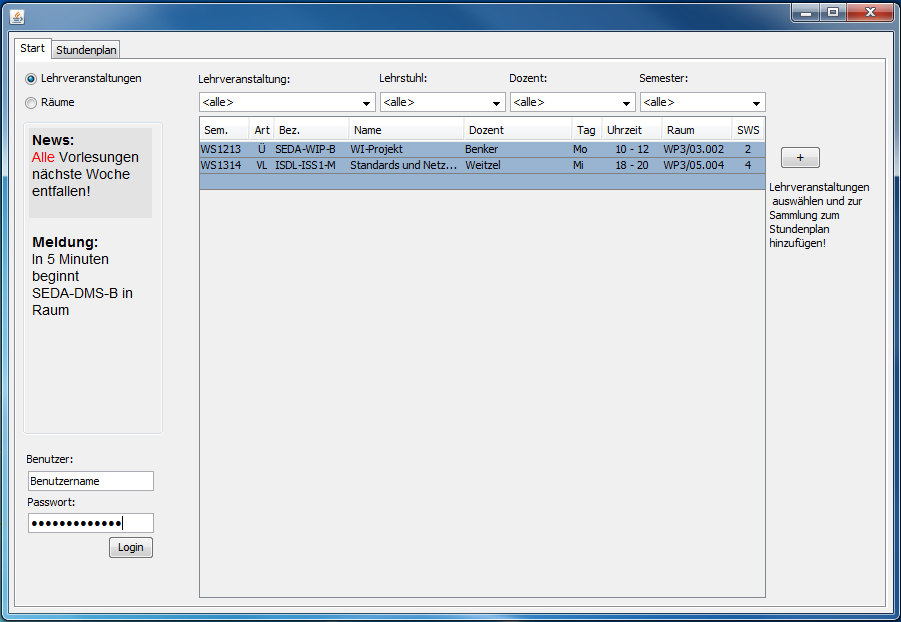
\includegraphics[width=170mm]{images/section_7/HauptseiteAlle.PNG}
\caption{GUI Startseite, rollenunabhängig}
\label{img:hauptseite}
\end{center}
\end{figure}

Im Falle einer erfolgreichen Anmeldung als Hausverwaltungsmitglied folgt die Startseite für Hausverwaltungsmitarbeiter. 
\begin{figure}[H]
\begin{center}
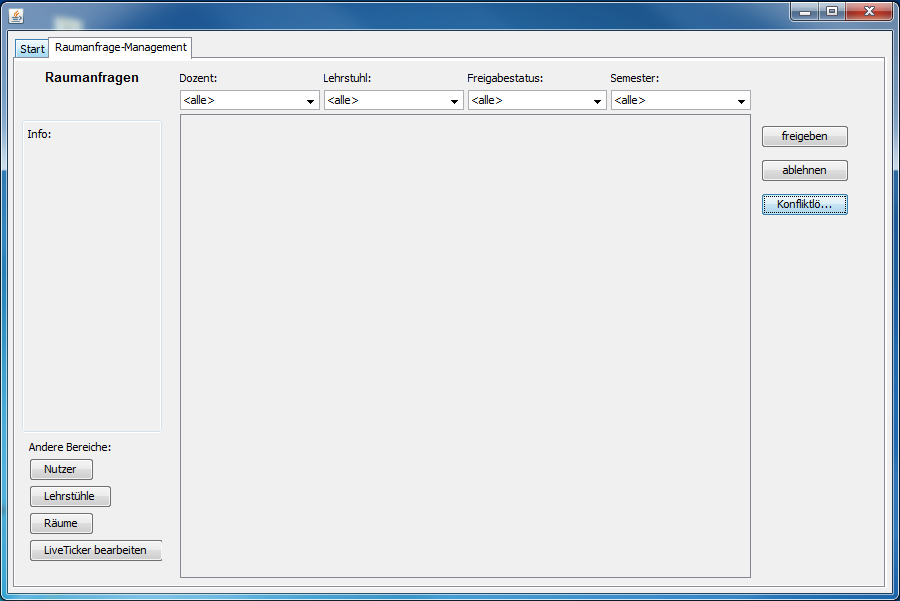
\includegraphics[width=170mm]{images/section_7/VerwaltungHauptseite.PNG}
\caption{Startseite für authentifizierte Benutzer der Hausverwaltung}
\label{img:hauptseiteVerwaltung}
\end{center}
\end{figure}
Sie haben einen unmittelbaren Überblick über alle Raumanfragen und können diese sogleich bearbeiten (freigeben, ablehnen oder etwaige Konflikte lösen, /F80/, /F40/).
Im linken Bereich ist Platz für einen personalisierten LiveTicker reserviert. Weiter unten können die Benutzer auf weitere Aktionen zugreifen.
\begin{figure}[H]
\begin{center}
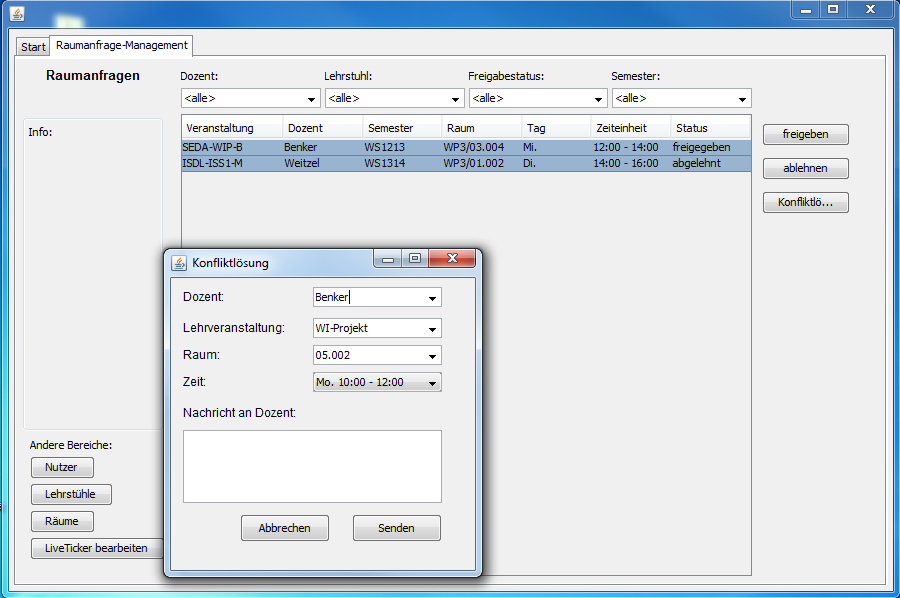
\includegraphics[width=170mm]{images/section_7/VerwaltungRaumanfragen.PNG}
\caption{Konfliktlösung der Raumanfragen}
\label{img:KonfliktlösungVerwaltung}
\end{center}
\end{figure}
Werden weitere Aktionen ausgeführt gelangt der Benutzer zu weiteren Listen und kann jeweils Lehrstühle, Nutzer und Räume verwalten (hinzufügen, bearbeiten oder löschen, /F10/, /F50/, /F51/, /F90/, /F100/). Bei der Raumverwaltung kann zusätzlich ein Raumplan erstellt werden (/F120/).
\begin{figure}[H]
\begin{center}
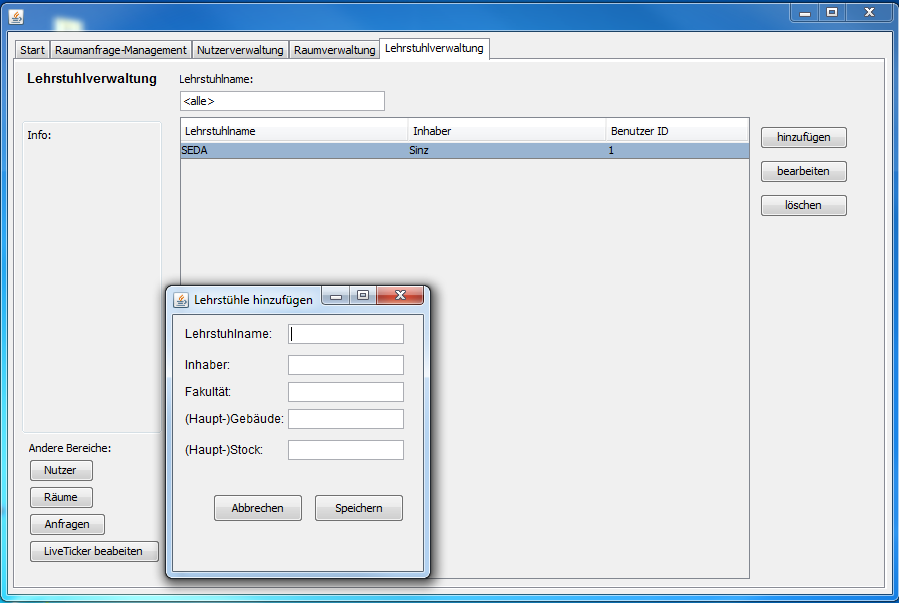
\includegraphics[width=170mm]{images/section_7/VerwaltungLehrstuhlverwaltung.PNG}
\caption{Verwaltung der Lehrstühle}
\label{img:LehrstuhlVerw}
\end{center}
\end{figure}

\begin{figure}[H]
\begin{center}
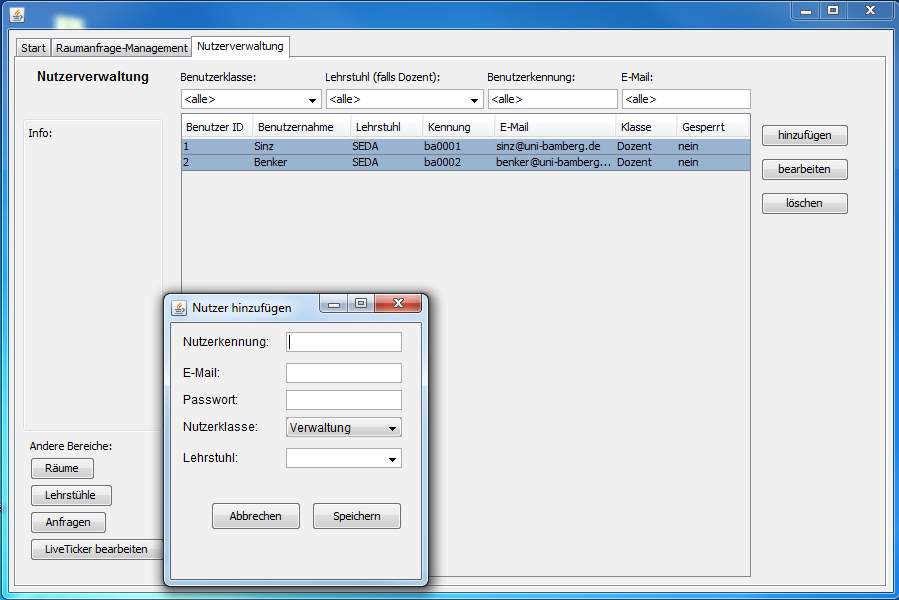
\includegraphics[width=170mm]{images/section_7/VerwaltungNutzerverwaltung.PNG}
\caption{Verwaltung der Nutzer}
\label{img:NutzerVerw}
\end{center}
\end{figure}

\begin{figure}[H]
\begin{center}
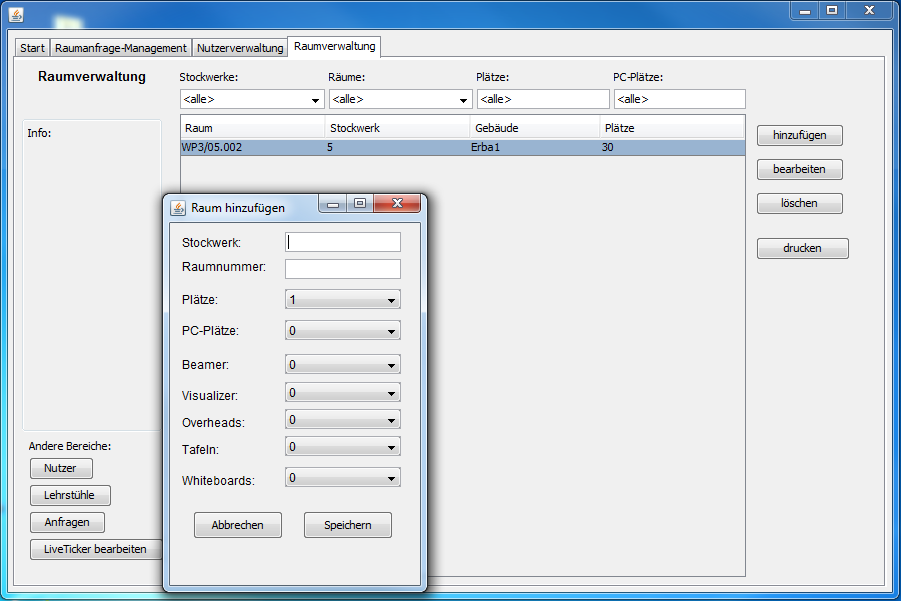
\includegraphics[width=170mm]{images/section_7/VerwaltungRaumverwaltung.PNG}
\caption{Verwaltung der Räume}
\label{img:RaumVerw}
\end{center}
\end{figure}
Eine letzte abdingbare Funktion wäre die Bearbeitung des LiveTickers um bspw. Dozenten verwaltungstechnische Nachrichten anzeigen lassen zu können (/FW21/).\\

Die personalisierte Startseite der Dozenten beinhaltet eine weiter Liste um alle Lehrveranstaltungen und besonderes den Status neu erstellter Lehrveranstaltungen anzeigen zu können (/F70/). Über den Veröffentlichungsstatus werden die bestätigten oder abgelehnten Raumanfragen angezeigt. Bei einer erfolgreich durchgeführten Raumanfrage kann der jeweilige Dozent seine Lehrveranstaltung anschließend veröffentlichen. Die mit der Raumanfrage bezogenen Nachrichten der Hausverwaltung werden im LiveTicker (links) angezeigt.
Außerdem können die Aktionen eigener Stundenplan (/F150/) und Lehrstuhlplan (/F140/) sowie eine LiveTicker Bearbeitung (um bspw. Studenten veranstaltungs- oder lehrstuhlsbezogene Nachrichten anzeigen lassen zu können, /FW21/) gewählt werden.
\begin{figure}[H]
\begin{center}
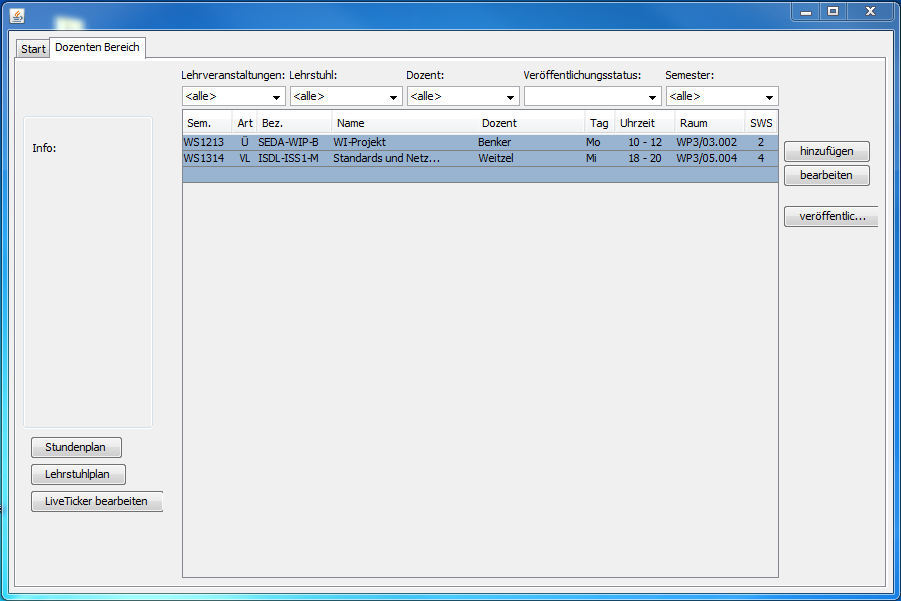
\includegraphics[width=170mm]{images/section_7/DozentenHauptseite.PNG}
\caption{Startseite für Dozenten}
\label{img:StartDoz}
\end{center}
\end{figure}
Um Lehrveranstaltungen zunächst überhaupt hinzuzufügen wird der Button "hinzufügen" gewählt und in einem neuen Fenster können Lehrstuhl und Dozent ausgewählt werden und somit die Bezeichnung der neuen Veranstaltung gesetzt werden (/F20/). Außerdem werden die benötigten Raumanforderungen für die Raumanfrage gewählt und alles zusammen versendet (/F30/). Die neue Veranstaltung wird der Liste hinzugefügt und die Raumanfrage an die Hausverwaltung zur weiteren Bearbeitung übermittelt.
\begin{figure}[H]
\begin{center}
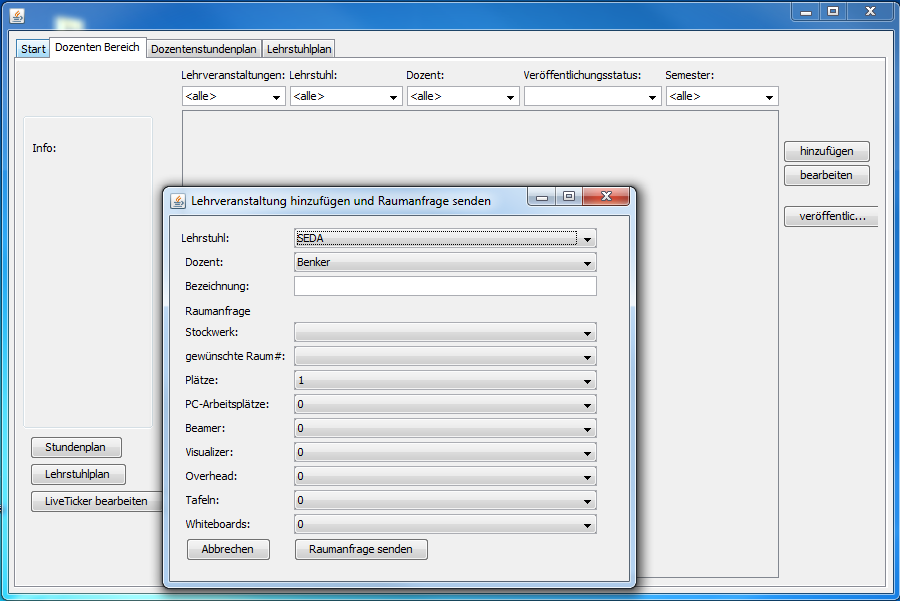
\includegraphics[width=170mm]{images/section_7/DozentenLehrveranstaltungeURaumanfrage.PNG}
\caption{Verwaltung der Lehrveranstaltungen und Raumanfragen durch die Dozenten}
\label{img:LehrveranstaltungsVerwDoz}
\end{center}
\end{figure}

